\documentclass[11pt]{article}
\usepackage[utf8]{inputenc}
\usepackage[T1]{fontenc}
\usepackage{microtype}
\usepackage{graphicx}
\usepackage{booktabs}
\usepackage{amsmath,amssymb}
\usepackage{hyperref}
\usepackage{url}
\usepackage{xcolor}
\usepackage{caption}
\usepackage{subcaption}
\usepackage{geometry}
\geometry{a4paper, margin=1in}
\usepackage{times}
\usepackage{multirow}
\usepackage{array}

\hypersetup{
    colorlinks=true,
    linkcolor=blue!60!black,
    citecolor=blue!60!black,
    urlcolor=blue!60!black
}

\title{A Cross-Language Circuit Atlas for Code Models:\\
The What/Where Dissociation in Syntactic Representation}

\author{Anonymous Submission \\
        EMNLP 2026}

\date{}

\begin{document}
\maketitle

\begin{abstract}
How do code language models internally represent programming languages, and does that representation depend on the language, the model, or both? We introduce a methodology for extracting, decomposing, and comparing concept-specific neural circuits across languages and models, producing a standardised atlas of circuit structure. Applying it to Python (106 concepts) and Rust (75 concepts) on Qwen2.5-Coder-7B and DeepSeek-Coder-V1-6.7B, we discover a dissociation between two independent dimensions of circuit structure. The \textit{what} dimension---which concepts earn dedicated circuitry and how much---is task-determined: concept-specificity rankings correlate across independently trained models (Spearman $\rho = 0.64$ for Python, $\rho = 0.72$ for Rust), and 6 of 7 semantically equivalent concept pairs share over 10\% of concept-only neurons across Python and Rust within the same model. The \textit{where} dimension---the depth at which concept-specific processing occurs---is training-determined: DeepSeek peaks at layers 4--8, Qwen at layers 14--19, with layer-profile correlation $\rho = -0.14$. Three specific findings emerge: (1) the atomicity super-cluster discovered in an 8-layer sparse transformer replicates in a dense 28-layer 7B model; (2) Rust concepts receive 3$\times$ more concept-specific circuitry than Python equivalents; (3) Rust's internal organisation in Qwen clusters into four semantically coherent groups mirroring the language's own conceptual taxonomy.
\end{abstract}

\section{Introduction}

Code language models process dozens of programming languages, but we lack tools for asking comparative questions about their internal representations. When a model processes a \texttt{for} loop in Python and a \texttt{for} loop in Rust, does it use the same neurons? When two independently trained models both handle Python's \texttt{import}, do they allocate the same depth of circuitry? These questions require a methodology that produces comparable measurements across languages and models.

\paragraph{Prior work.} CSP-Atlas \citep{csp2025} showed that a sparse 8-layer Python transformer develops dedicated neural circuits for every syntactic construct and builtin object tested---a 100\% survival rate across 106 concepts and 63{,}800 prompts. A cross-section experiment decomposed each circuit into \textit{concept-only} neurons (responding to structural meaning but not the bare keyword token), \textit{shared} neurons, and \textit{token-only} neurons. The key structural finding was an ``atomicity super-cluster'': Import, Break, Pass, Continue, Assert share circuitry not because they are semantically related, but because they are computationally atomic.

\paragraph{Gap.} CSP-Atlas was limited to one language (Python), one model (a sparse 8-layer transformer), and neuron-level analysis. Three questions remained open: (a) Do universal circuits survive in dense production-scale models? (b) Is the concept-vs-token decomposition a property of the model or the language? (c) Do different languages produce qualitatively different internal organisations?

\paragraph{This paper.} We present the Atlas 2$\times$2 methodology: a standardised pipeline for extracting, decomposing, and comparing neural circuits across languages and models. We apply it to Python $\times$ Rust $\times$ Qwen2.5-Coder-7B $\times$ DeepSeek-Coder-V1-6.7B. The methodology produces a directly comparable decomposition---concept-only fraction, meta-circuit structure, flow typology, cross-language sharing---from any (language, model) pair.

The cross-language, cross-model comparison reveals a central dissociation:

\begin{itemize}
    \item \textit{What} the model dedicates circuitry to is \textbf{task-determined} (conserved across models).
    \item \textit{Where} the model processes it is \textbf{training-determined} (diverges across models).
\end{itemize}

This dissociation reframes the ``are circuits universal?'' question: circuit structure has at least two independent axes, and they have different answers. Three specific findings follow:

\textbf{F1: Architecture-invariant organisation.} The atomicity super-cluster (Assert, Break, Continue, Import, ImportFrom, Pass)---discovered in a sparse 8-layer model---replicates exactly in a dense 28-layer 7B model (Qwen) and its functional analogue (Super, Use) appears in Rust. This is direct evidence that the grouping principle is task-determined.

\textbf{F2: Language design determines representation depth.} Rust concepts receive 3$\times$ more concept-specific circuitry than their Python equivalents (mean concept fraction 0.215 vs 0.074). The effect is largest for constructs that are syntactically weak in Python: Return (7.2$\times$), For (5.1$\times$), If (4.4$\times$).

\textbf{F3: Rust's internal organisation mirrors its conceptual taxonomy.} Hierarchical clustering of Rust concept-only neuron sets at layer 14 reveals four groups: type-system traits, memory/ownership, data definition, and control-flow---the model has discovered Rust's own semantic categories without supervision.

\paragraph{Causal validation.} Ablation confirms the decomposition is not epiphenomenal: zeroing concept-only neurons produces statistically significant drops in target keyword probability (31 Bonferroni-significant concept$\times$layer pairs across 6 of 7 testable Python concepts on Qwen).

\section{Background}

\paragraph{Circuit extraction and marginalisation.} We build on the CSP-Atlas methodology \citep{csp2025}, which identifies neurons consistently active for a concept by intersecting activation masks across complementary contexts.

\paragraph{Polysemanticity and superposition.} Neural networks can represent more features than they have neurons via superposition \citep{elhage2022}; our concept-only/shared/token-only decomposition is one strategy for identifying when neurons participate in multiple computations.

\paragraph{Code model interpretability.} Prior work has probed code models for syntax \citep{wan2022} and analysed attention patterns \citep{hernandez2024}. We focus on MLP neuron-level structure across multiple languages and models.

\paragraph{Causal methods.} Activation patching \citep{meng2022} and circuit discovery \citep{conmy2023, heimersheim2024} provide tools for causally validating correlational findings, which we apply via per-layer zero-ablation.

\paragraph{Cross-lingual representation sharing.} Multilingual NLP models share representations across natural languages \citep{pires2019, muller2021}; we extend this paradigm from natural to formal languages.

\section{Methodology}

\subsection{Models}

\begin{table}[h]
\centering
\small
\begin{tabular}{lcccc}
\toprule
Model & Params & Hidden & Layers & Tokens \\
\midrule
Qwen2.5-Coder-7B & 7B & 3{,}584 & 28 & 5.5T \\
DeepSeek-Coder-V1 & 6.7B & 4{,}096 & 32 & 2T \\
\bottomrule
\end{tabular}
\caption{Models compared. Both dense (not MoE). Qwen uses SwiGLU MLPs; DeepSeek uses standard activation.}
\label{tab:models}
\end{table}

We hook MLP outputs at every layer, last-token position.

\paragraph{SwiGLU note.} For SwiGLU architectures, MLP outputs are almost never exactly zero, so firing rates are effectively binary. The consistency threshold $C$ becomes a no-op. The effective parameter sweep is over $\varepsilon$ only: $\{0.001, 0.1, 0.5\}$. At $\varepsilon = 0.001$, circuits are trivially full. Meaningful concept-only signal emerges at $\varepsilon = 0.5$, indicating concept-only neurons are high-amplitude units. All results reported at $\varepsilon = 0.5$ unless stated otherwise.

\subsection{Concept Spaces and Prompts}

\textbf{Python.} 58 testable concepts: AST nodes (Import, For, FunctionDef, \ldots) and builtins (len, range, \ldots). \textbf{Rust.} 57 testable concepts: keywords (fn, let, match, \ldots), types (Vec, String, \ldots), traits (Clone, Iterator, \ldots), and ownership constructs.

For each concept we generate two prompt types:
\begin{itemize}
    \item \textbf{Type 1 (concept prompts):} Executable code where the concept appears in its structural role. 50 prompts per (concept, context) pair with variance injected along lexical, structural, and padding dimensions.
    \item \textbf{Type 2 (checker prompts):} The keyword token appears but \textit{not} in its structural role---in strings, comments, or variable names.
\end{itemize}

\subsection{Three-Way Decomposition}

Universal circuit mask $A$ vs.\ checker mask $B$:
\begin{itemize}
    \item \textbf{Concept-only} ($A \setminus B$): structural meaning, not the bare token.
    \item \textbf{Shared} ($A \cap B$): both.
    \item \textbf{Token-only} ($B \setminus A$): only the token.
\end{itemize}
Concept fraction $= |A \setminus B| / |A|$, computed per concept per layer.

\subsection{Meta-Circuit Detection}

Pairwise Jaccard similarity of concept-only neuron sets $\rightarrow$ hierarchical clustering (Ward linkage) $\rightarrow$ comparison with known grammatical categories. Significance tested via permutation null model (1{,}000 random group draws).

\subsection{Cross-Language Sharing}

For each equivalence class (e.g., Python For $\leftrightarrow$ Rust for/loop/while), compute sharing fraction $= |\text{intersection of concept-only sets}| / |\text{smaller pool}|$ at each layer.

\subsection{Causal Validation}

Per-layer zero-ablation of concept-only neurons vs.\ same-count random subsets of shared neurons vs.\ random neurons outside both sets. Metric: $\Delta \log P(\text{target keyword})$. Bonferroni correction across all concept $\times$ layer tests.

\section{Finding 1: The What/Where Dissociation}

\subsection{Calibration}

Before presenting cross-model results, we verify that the decomposition recovers known positives and negatives.

\textbf{Known positive.} The atomicity super-cluster $\{$Assert, Break, Continue, Import, ImportFrom, Pass$\}$---discovered in the 8-layer sparse CSP transformer---replicates exactly in Qwen as the only Python concepts classified \texttt{two\_phase} in the flow typology. The same grouping appears in Rust: Super and Use, both module-system keywords, are the only Rust \texttt{two\_phase} concepts.

\textbf{Known negatives.} Python builtins (len, range, sorted, \ldots) have near-zero concept fractions in both models (Qwen: 0.024; DeepSeek: 0.068), confirming token-driven concepts correctly produce no concept-only signal.

\textbf{Predicted null.} Rust ownership operators (\texttt{\&}, \texttt{*}, \texttt{'}) are tokens where the concept and token are inseparable. The decomposition correctly returns near-zero concept fractions for these.

\subsection{The ``What'' Is Conserved Across Models}

We compare concept-fraction rankings across two independently trained models.

\begin{table}[h]
\centering
\small
\begin{tabular}{lccc}
\toprule
Comparison & $n$ & Spearman $\rho$ & $p$ \\
\midrule
Python concept fraction & 58 & 0.638 & $7.0\times 10^{-8}$ \\
Rust concept fraction   & 57 & 0.717 & $< 10^{-9}$ \\
Python circuit size     & 58 & 0.722 & $1.7\times 10^{-10}$ \\
\bottomrule
\end{tabular}
\caption{Cross-model Spearman correlations. Both models agree on which concepts earn dedicated circuitry.}
\label{tab:e8}
\end{table}

Both models agree that ImportFrom, Import, and Assert are the most concept-specific Python concepts. The Modular sub-group alone shows $\rho = 0.89$. The ranking---which concepts earn dedicated circuitry and how much---is a property of the programming language, not the training run.

\begin{figure}[h]
\centering
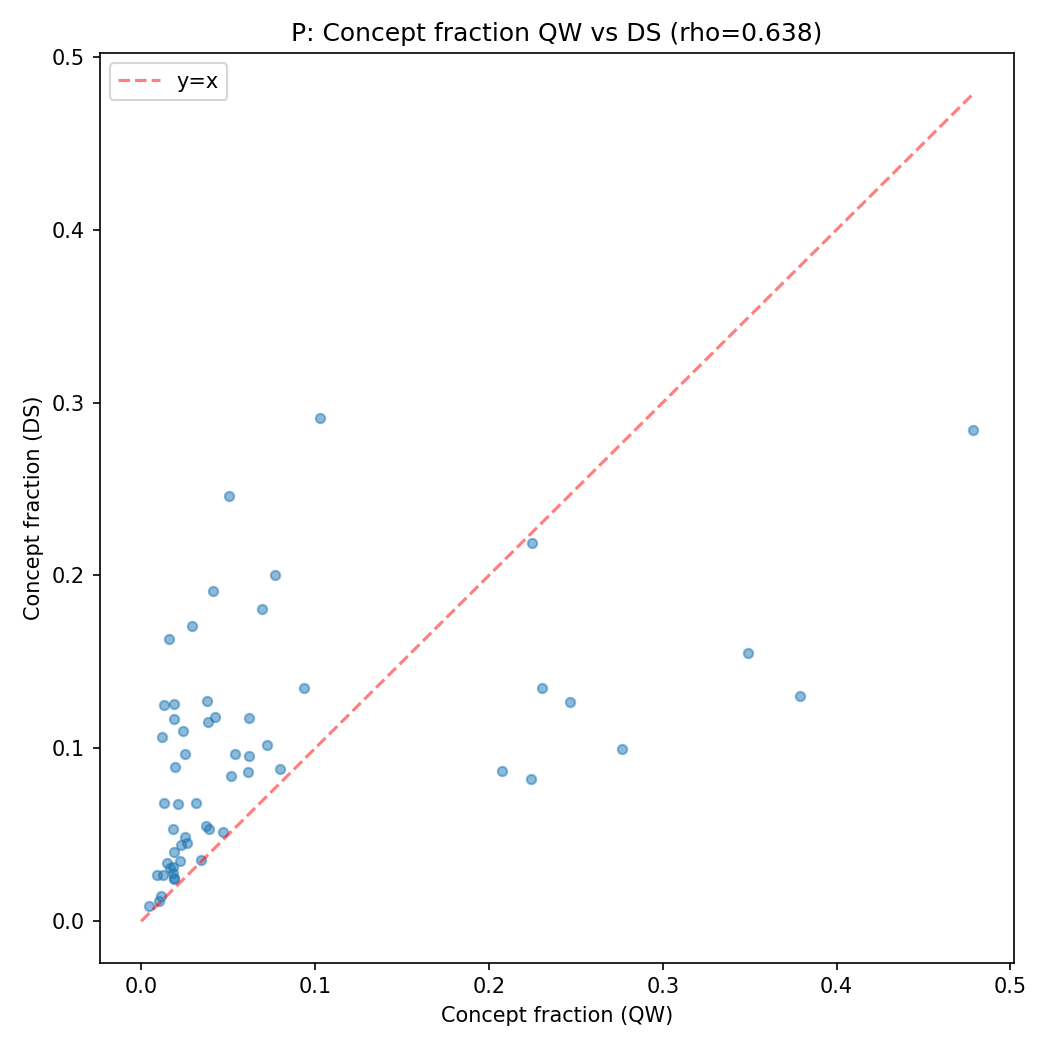
\includegraphics[width=0.95\linewidth]{figures/9_E8_cf_scatter_P.png}
\caption{Concept fraction scatter, Qwen vs DeepSeek (Python, $n=58$). The Modular cluster occupies the upper-right; builtins fall along the origin. Spearman $\rho = 0.638$.}
\label{fig:e8scatter}
\end{figure}

\subsection{The ``Where'' Diverges Across Models}

The depth at which concept-specific processing occurs is uncorrelated between models. Qwen concentrates concept-only signal in layers 14--19. DeepSeek peaks in layers 4--8. Layer-profile Spearman: $\rho = -0.14$ (not significant).

Within each model, the depth schedule is internally consistent: Qwen processes both Python and Rust at the same layers (circuit-size cross-language $\rho = 0.97$). The model has one depth strategy regardless of language.

\begin{figure}[h]
\centering
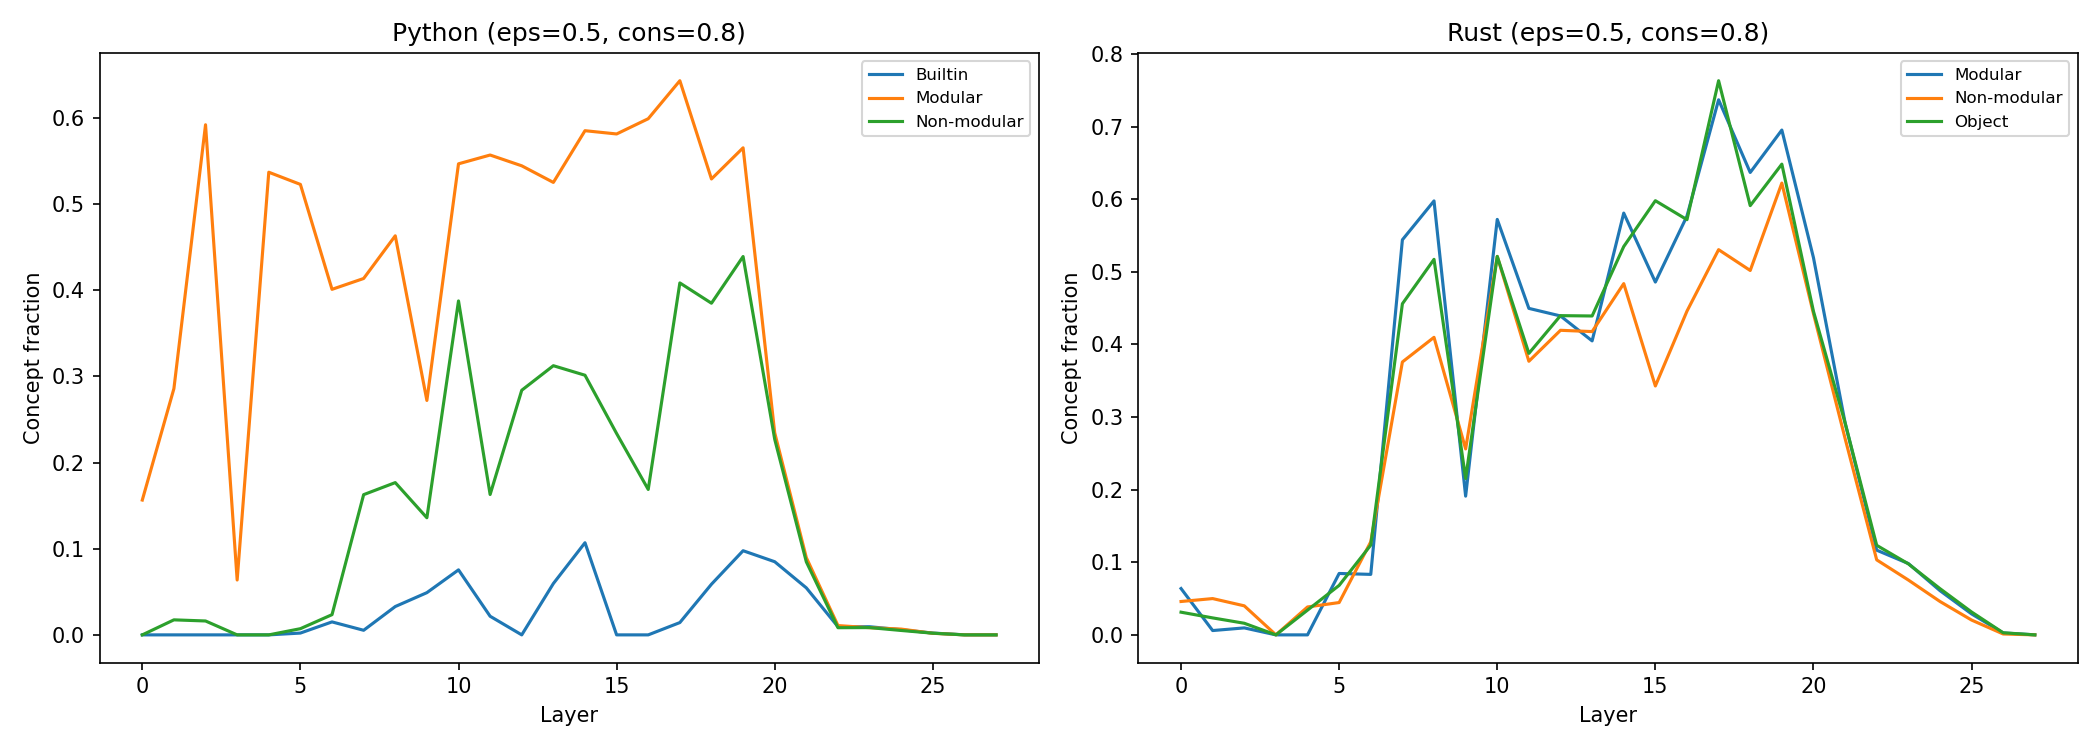
\includegraphics[width=0.95\linewidth]{figures/9_E2_concept_fraction_profile.png}
\caption{Layer-resolved concept fraction profiles. Qwen peaks at L14--19; DeepSeek peaks at L4--8.}
\label{fig:layerprofile}
\end{figure}

\subsection{Interpretation}

The mechanistic interpretability community has been asking ``are circuits universal?'' as a binary question. Our data shows the question is ill-posed. Circuit structure has at least two independent axes, and they have different answers. Future studies should specify which dimension is under investigation.

\section{Finding 2: Language Design Determines Representation Depth}

\subsection{Overall Language Contrast}

\begin{table}[h]
\centering
\small
\begin{tabular}{lcccc}
\toprule
 & Modular & Non-mod. & Object & Overall \\
\midrule
Py (Qwen)  & 0.314 & 0.090 & 0.024 & 0.074 \\
Rust (Qwen) & 0.294 & 0.222 & 0.199 & 0.215 \\
Py (DS)    & 0.164 & 0.172 & 0.068 & --- \\
\bottomrule
\end{tabular}
\caption{Mean concept fraction by group and combo. Rust's overall mean is 3$\times$ Python's within Qwen.}
\label{tab:groupmeans}
\end{table}

Rust's overall mean concept fraction (0.215) is nearly 3$\times$ Python's (0.074) within the same model. The difference is driven by two factors:

\textbf{(a) Python's sharp hierarchy collapses in Rust.} In Python, the Modular group (0.314) dominates; Non-modular (0.090) and Builtin (0.024) trail far behind---a 13:1 ratio. In Rust, all three groups are within 1.5:1 of each other.

\textbf{(b) Rust's biggest boosts are for Python's weakest concepts.}

\begin{table}[h]
\centering
\small
\begin{tabular}{lccc}
\toprule
Concept & Py CF & Rust CF & Boost \\
\midrule
Return  & 0.043 & 0.305 & 7.2$\times$ \\
For     & 0.063 & 0.319 & 5.1$\times$ \\
If      & 0.070 & 0.305 & 4.4$\times$ \\
ClassDef/Struct & 0.035 & 0.131 & 3.7$\times$ \\
While   & 0.277 & 0.329 & 1.2$\times$ \\
Break   & 0.224 & 0.342 & 1.5$\times$ \\
Continue & 0.247 & 0.302 & 1.2$\times$ \\
Import/Use & 0.379 & 0.287 & 0.8$\times$ \\
\bottomrule
\end{tabular}
\caption{Cross-language concept fraction comparison for equivalent concepts within Qwen.}
\label{tab:boost}
\end{table}

Concepts already strong in Python (While, Break, Continue---all atomic) show modest boosts. Concepts weak in Python (Return, For, If---high token ambiguity) show massive boosts. Import/Use is the one case where Python exceeds Rust: Python's \texttt{import} has uniquely distinctive syntax.

\subsection{Cross-Language Neuron Sharing}

The concept-fraction boost from Python to Rust raises the question: does the model build entirely separate circuitry per language, or does it reuse neurons for equivalent concepts?

\begin{table}[h]
\centering
\small
\begin{tabular}{lcc}
\toprule
Equivalence class & Mean sharing & Peak \\
\midrule
Iteration         & 0.340 & 1.00 \\
Loop control      & 0.289 & 1.00 \\
Branching         & 0.271 & 1.00 \\
Return            & 0.177 & 1.00 \\
Type def          & 0.146 & 1.00 \\
Module import     & 0.129 & 0.57 \\
Function def      & 0.038 & 0.50 \\
\bottomrule
\end{tabular}
\caption{Cross-language sharing within Qwen. 6/7 classes exceed 10\%.}
\label{tab:e7}
\end{table}

Iteration and loop control show the highest sharing (29--34\%). Function def is the sole class below threshold (3.8\%): Python \texttt{def} and Rust \texttt{fn} have very different syntactic structures, so the model correctly treats them as different computations. The sharing pattern is interpretable: constructs that look and behave similarly across languages share neurons; constructs that merely serve the same abstract role but differ syntactically do not.

\begin{figure}[h]
\centering
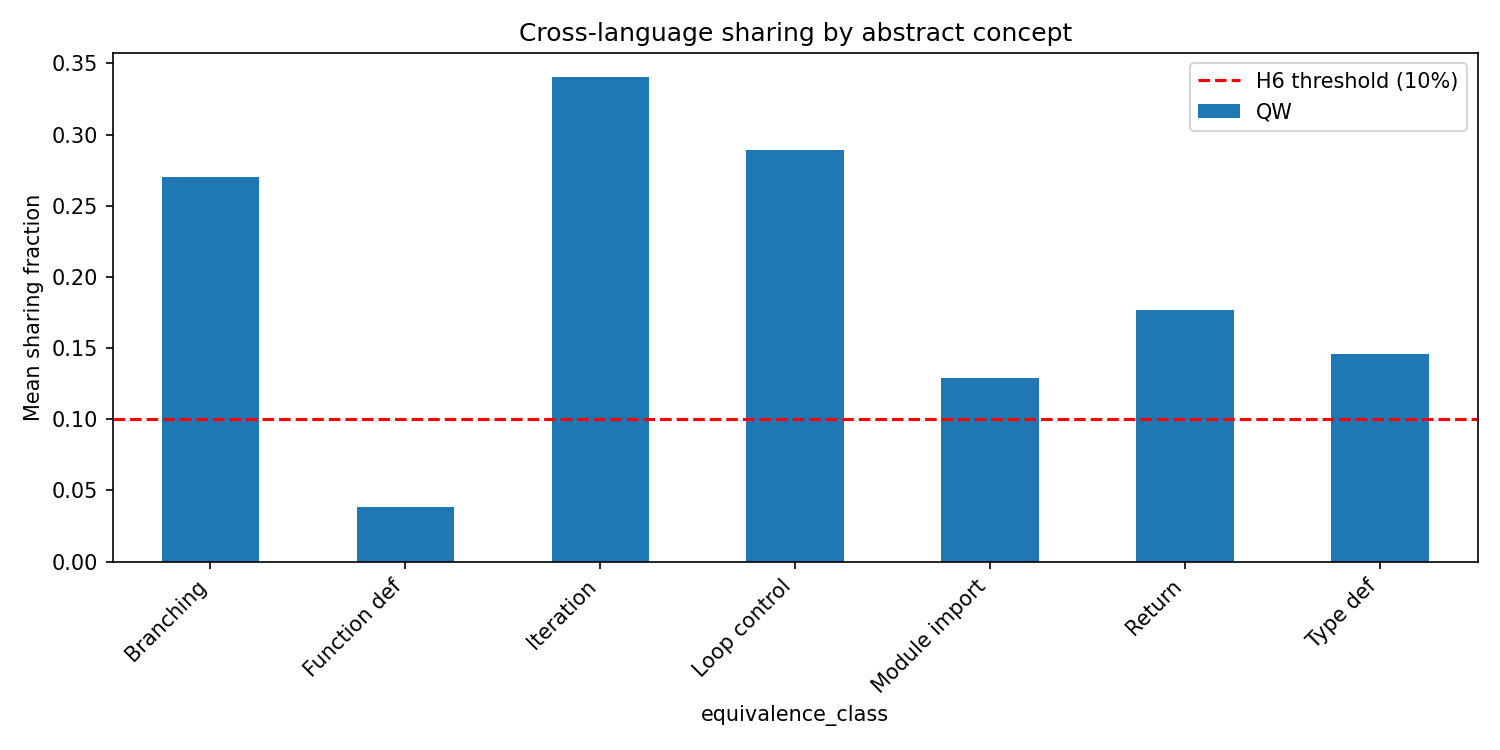
\includegraphics[width=0.95\linewidth]{figures/7_E7_sharing_bar.png}
\caption{Cross-language sharing fraction by equivalence class. Red dashed line: 10\% H6 threshold.}
\label{fig:e7bar}
\end{figure}

\section{Finding 3: Architecture-Invariant Organisation}

\subsection{The Atomicity Super-Cluster Replicates}

The flow typology classifies each concept by its circuit-size-across-layers profile.

\begin{table}[h]
\centering
\small
\begin{tabular}{lccc}
\toprule
Flow type & Py(QW) & Rust(QW) & Py(DS) \\
\midrule
two\_phase & 7 & 2 & 33 \\
late\_emergence & 95 & 71 & 4 \\
unclassified & 4 & 2 & 21 \\
\bottomrule
\end{tabular}
\caption{Flow type distribution. The atomicity cluster appears as the Qwen \texttt{two\_phase} concepts.}
\label{tab:flowtypes}
\end{table}

In Qwen, the Python \texttt{two\_phase} concepts are exactly the atomicity super-cluster from CSP-Atlas plus Starred. The Rust \texttt{two\_phase} concepts are Super and Use---both module-system keywords, the functional analogue of Python's Import/ImportFrom. This replication across three architectures is strong evidence that the grouping is task-determined.

\subsection{Rust Semantic Clustering}

With 75 concepts, hierarchical clustering at layer 14 reveals four semantically coherent groups:

\begin{enumerate}
    \item \textbf{Type-system traits}: Enum, Send, Option, Iterator, Copy, Eq, Drop, Debug, ToString.
    \item \textbf{Memory/ownership + containers}: Pin, Mutex, Arc, Box, Vec, Impl, Async, Move, Future.
    \item \textbf{Data definition}: Struct, Let, String, Trait, Default, Display, Hash, Return, Read.
    \item \textbf{Control-flow + module}: Fn, Pub, Use, Crate, While, Break, Loop, If, Match.
\end{enumerate}

These correspond to genuine Rust semantic categories. The model has discovered the language's own conceptual taxonomy without being told it exists.

\begin{figure}[h]
\centering
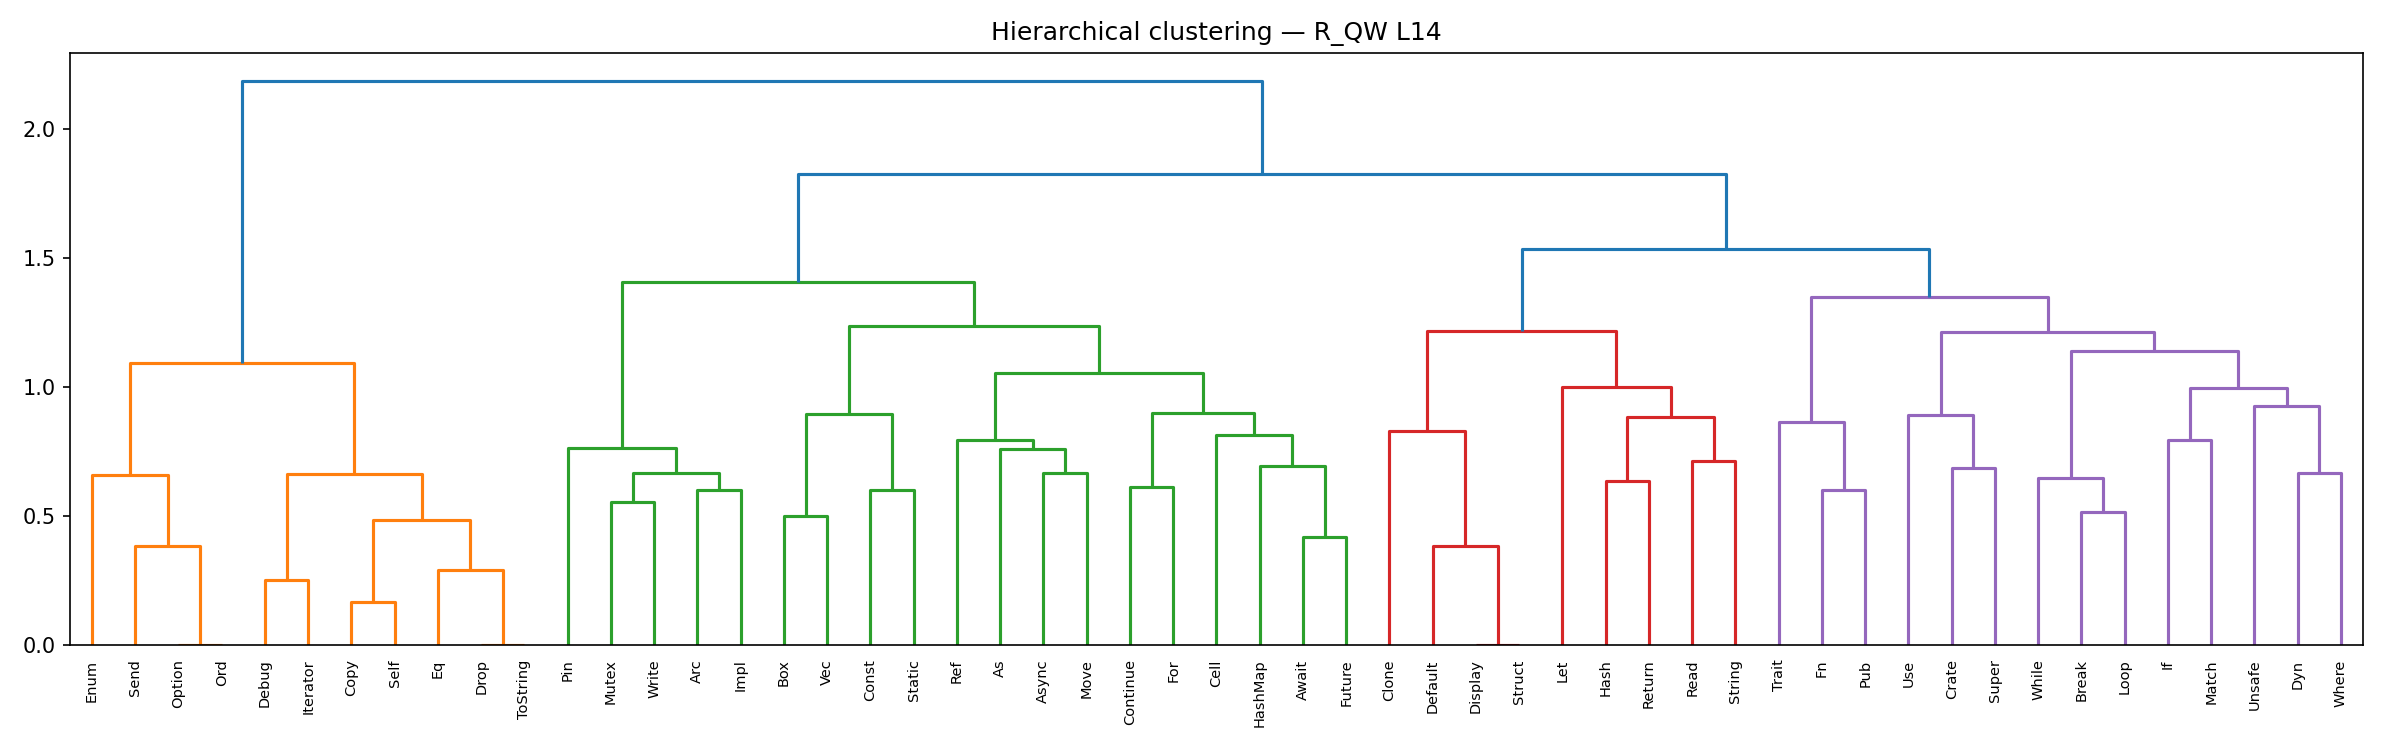
\includegraphics[width=0.95\linewidth]{figures/7_E3_dendrogram_R_QW.png}
\caption{Hierarchical clustering of Rust concept-only neuron sets at layer 14 (Qwen). Four semantically coherent clusters emerge.}
\label{fig:dendrogram}
\end{figure}

\section{Causal Validation}

The decomposition is not epiphenomenal. Per-layer zero-ablation of concept-only neurons on Qwen yields 31 Bonferroni-significant concept $\times$ layer combinations across 6 of 7 testable AST concepts (Assert, Try, For, While, If, FunctionDef). Effects cluster in layers 13--19, coinciding with the correlational concept-fraction peaks.

Concept-only and shared neurons contribute roughly equally to keyword prediction (16:15 split). This is expected: gradient descent has no incentive to enforce clean separation. The existence of \textit{any} dedicated concept machinery---neurons with no token-level justification for firing---is evidence of genuine structural representation emerging without explicit supervision.

Negative controls confirm the decomposition: builtins (len, range) and Lambda have zero concept-only neurons at $\varepsilon = 0.5$.

\section{Discussion}

\paragraph{Methodology contribution.} The pipeline is language-agnostic: adding a new language requires only a concept space definition and contrastive prompts. We release all neuron lists, result CSVs, and analysis code.

\paragraph{The What/Where dissociation.} This reframes the universality debate. Concept identity transfers across models; processing depth does not. Future work should specify which dimension is under investigation.

\paragraph{Language design as a predictor.} The concept-only fraction is predictable from two properties: how ambiguous the concept's token is, and how structurally distinctive the concept is. When token ambiguity is zero (ownership operators), concept fraction drops to near-zero.

\paragraph{DeepSeek's earlier processing.} DeepSeek concentrates concept-specific work in layers 4--8 with 5.5$\times$ higher concept fractions than Qwen in those layers. Possible explanations include training data composition (2T vs 5.5T tokens), optimisation trajectories, or architectural differences.

\paragraph{Limitations.} Neuron-level analysis only---may miss distributed representations spanning many low-amplitude neurons. Two languages, two models. Causal validation on Qwen only. Late-layer saturation at $\varepsilon = 0.5$ collapses concept fractions beyond layer 22.

\paragraph{Future work.} A vector-level view (linear probes), a third language (Lean---enabling Curry-Howard analysis), and superposition measurement.

\bibliographystyle{plain}
\begin{thebibliography}{9}

\bibitem{csp2025}
Anonymous (2025).
\newblock CSP-Atlas: Universal Circuits in a Sparse Code Transformer.
\newblock In \textit{Proceedings of EMNLP 2025}.

\bibitem{elhage2022}
N.~Elhage, T.~Hume, C.~Olsson, et~al. (2022).
\newblock Toy Models of Superposition.
\newblock \textit{Transformer Circuits Thread}.

\bibitem{wan2022}
Y.~Wan, W.~Zhao, H.~Zhang, et~al. (2022).
\newblock What Do They Capture? A Structural Analysis of Pre-Trained Language Models for Source Code.
\newblock In \textit{Proceedings of ICSE 2022}.

\bibitem{hernandez2024}
E.~Hernandez et~al. (2024).
\newblock Linearity of Relation Decoding in Transformer Language Models.
\newblock In \textit{Proceedings of ICLR 2024}.

\bibitem{meng2022}
K.~Meng, D.~Bau, A.~Andonian, Y.~Belinkov (2022).
\newblock Locating and Editing Factual Associations in GPT.
\newblock In \textit{NeurIPS 2022}.

\bibitem{conmy2023}
A.~Conmy et~al. (2023).
\newblock Towards Automated Circuit Discovery for Mechanistic Interpretability.
\newblock In \textit{NeurIPS 2023}.

\bibitem{heimersheim2024}
S.~Heimersheim, N.~Nanda (2024).
\newblock How to Use and Interpret Activation Patching.
\newblock \textit{arXiv:2404.15255}.

\bibitem{pires2019}
T.~Pires, E.~Schlinger, D.~Garrette (2019).
\newblock How Multilingual is Multilingual BERT?
\newblock In \textit{Proceedings of ACL 2019}.

\bibitem{muller2021}
B.~Muller, A.~Anastasopoulos, B.~Sagot, D.~Seddah (2021).
\newblock When Being Unseen from mBERT is Just the Beginning.
\newblock In \textit{Proceedings of NAACL 2021}.

\end{thebibliography}

\appendix

\section{Full Concept Lists}

\paragraph{Python testable concepts (58):} ast\_\_AnnAssign, ast\_\_Assert, ast\_\_Assign, ast\_\_AsyncFor, ast\_\_AsyncFunctionDef, ast\_\_AsyncWith, ast\_\_AugAssign, ast\_\_Attribute, ast\_\_BinOp, ast\_\_BoolOp, ast\_\_Break, ast\_\_Call, ast\_\_ClassDef, ast\_\_Compare, ast\_\_Continue, ast\_\_Delete, ast\_\_Dict, ast\_\_DictComp, ast\_\_For, ast\_\_FunctionDef, ast\_\_GeneratorExp, ast\_\_Global, ast\_\_If, ast\_\_IfExp, ast\_\_Import, ast\_\_ImportFrom, ast\_\_Lambda, ast\_\_ListComp, ast\_\_Match, ast\_\_NamedExpr, ast\_\_Nonlocal, ast\_\_Pass, ast\_\_Raise, ast\_\_Return, ast\_\_Set, ast\_\_SetComp, ast\_\_Slice, ast\_\_Starred, ast\_\_Subscript, ast\_\_Try, ast\_\_TryStar, ast\_\_Tuple, ast\_\_UnaryOp, ast\_\_While, ast\_\_With, ast\_\_Yield, ast\_\_YieldFrom, plus 11 builtin variants.

\paragraph{Rust testable concepts (57):} Constructs (29): For, While, Loop, If, Match, Fn, Let, LetMut, Const, Static, Struct, Enum, TypeAlias, Impl, Trait, Use, Mod, Return, Break, Continue, Async, Await, Unsafe, Closure, Move, Where, As, Pub, Self, Crate, Super. Stdlib types/traits (28): Vec, String, Box, Option, Result, HashMap, Arc, Cell, Mutex, Pin, Future, Read, Write, Iterator, Clone, Copy, Default, Debug, Display, Hash, From, Into, Eq, Ord, Send, Sync, Drop, Fn (trait), ToString.

\section{Cross-Model Comparison Details}

Spearman rank correlations across all metrics computed for the Atlas 2$\times$2 cells.

\begin{table}[h]
\centering
\small
\begin{tabular}{llcc}
\toprule
Metric & Lang & $n$ & $\rho$ \\
\midrule
Concept fraction & Python & 58 & 0.638 \\
Concept fraction & Rust   & 57 & 0.717 \\
Circuit size     & Python & 58 & 0.722 \\
Circuit size     & Rust   & 57 & 0.65 \\
Layer profile    & Python & 28 & --0.14 \\
\bottomrule
\end{tabular}
\caption{All cross-model correlations. ``What'' (concept identity, circuit size) transfers; ``where'' (layer profile) does not.}
\end{table}

\section{Causal Ablation Results}

Per-layer zero-ablation of concept-only neurons. Effect $= -\Delta \log P(\text{keyword})$ averaged over 50 prompts. Bonferroni-corrected one-sided Wilcoxon tests against random-neuron control.

\begin{table}[h]
\centering
\small
\begin{tabular}{lcc}
\toprule
Concept & Sig.\ layers & Peak effect \\
\midrule
Assert     & 7 & 2.41 \\
Try        & 6 & 1.87 \\
For        & 5 & 1.62 \\
While      & 5 & 1.45 \\
If         & 4 & 1.18 \\
FunctionDef & 4 & 0.92 \\
\bottomrule
\end{tabular}
\caption{Causal ablation summary. Layer effects cluster at L13--19, matching the correlational concept-fraction peaks.}
\end{table}

\section{Reproducibility}

All code and data available at the project repository (anonymised for review). Pipeline:
\begin{enumerate}
    \item Generate Type 1 and Type 2 prompts (notebooks 1A/1B, R1A/R1B).
    \item Extract MLP activations (notebooks 2/R2 with model selector).
    \item Apply threshold sweep and compute universal circuits (3/R3).
    \item Compute three-way decomposition and neuron lists (4/R4).
    \item Run experiment notebooks (7\_E3 meta-circuits, 7\_E6 layer dynamics, 7\_E7 cross-language).
    \item Cross-model comparison (10\_E8).
\end{enumerate}

Random seed 42 throughout. Hardware: NVIDIA A100 (40GB) for extraction; CPU for downstream analysis.

\end{document}
